\documentclass{if-beamer}

% --------------------------------------------------- %
%                  Presentation info	              %
% --------------------------------------------------- %
\title[Lecture 4]{Lecture 4}
\subtitle{Using the Unix Shell and Introduction to C++}
\author{Instructor: Ashley Gannon}
\date{ISC3313 Fall 2021}
\logo{

\includegraphics[scale=0.08]{figures/FSULogo.png}
}
\subject{Presentation subject} % metadata

\graphicspath{{figures/}}
% --------------------------------------------------- %
%                    Title + Schedule                 %
% --------------------------------------------------- %
\begin{document}

\begin{frame}
  \titlepage
\end{frame}
% --------------------------------------------------- %
%                      Presentation                   %
% --------------------------------------------------- %
\section{Unix shell and Basic Commands}

\begin{frame}
\frametitle{Using the Unix Shell}
When we open the Bash shell (Windows), or the iTerm (Mac),
we are first presented with a prompt:
\begin{figure}
	\center
	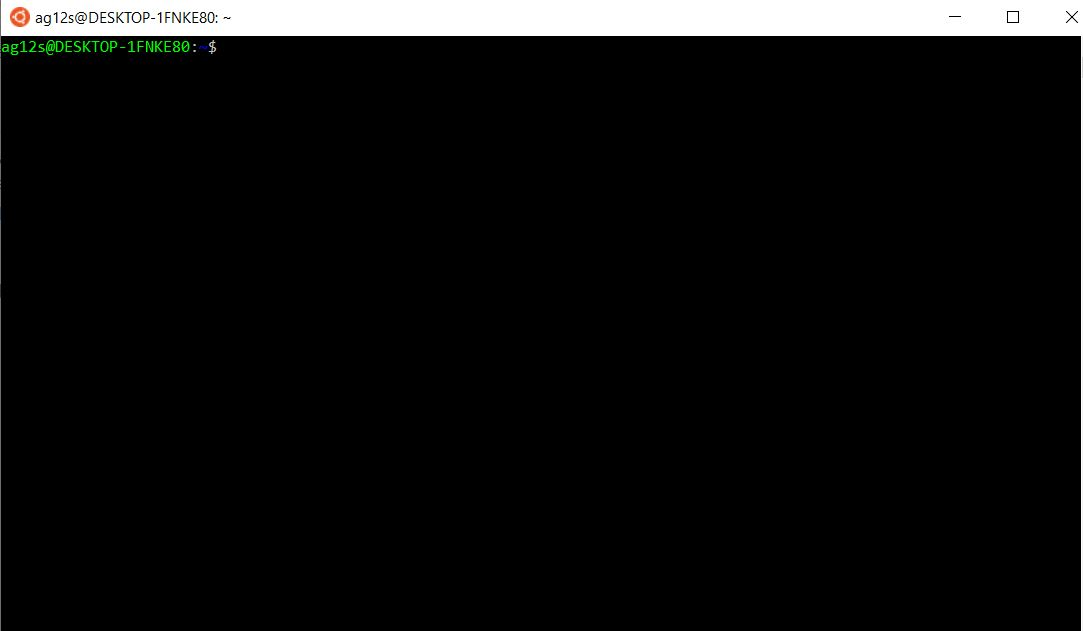
\includegraphics[width=0.8\textwidth]{bashwindow.jpg}
\end{figure}
Here we can enter many commands recognized by the Shell language.
\end{frame} 

\begin{frame}
\frametitle{Basic Commands}
Here are some of the most basic commands:
\begin{itemize}
\item \texttt{ls}: list the contents of the current directory
\item \texttt{pwd}: display the current path from root
\item \texttt{cd}: change directory
\item \texttt{cp}: copy a file/directory
\item \texttt{rm}: delete (or remove) a file/directory
\item \texttt{mv}: move a file/directory to a different name/path
\item \texttt{touch}: create (or make) a file
\item \texttt{mkdir}: create (or make) a directory
\end{itemize}
\end{frame}

\begin{frame}
\frametitle{Special symbols}
There are some special symbols that a user just \textit{must} be
familiar with:
\begin{itemize}
\item \texttt{.}: the period stands for 'current directory'
\item \texttt{..}: two periods stand for 'previous directory'
\item \texttt{/}: forward slash stands for 'root directory'
\item \texttt{\textasciitilde}: tilde stands for 'home directory'
\end{itemize}
\end{frame}

\begin{frame}
\frametitle{Beyond Navigation of Directories}
We can interact with the Shell in many ways. We can define variables,
view files, open a program for file editing, or do simple math right in
our terminal! Here are some simple commands:
\begin{itemize}
\item \texttt{echo}: display argument to string or file
\item \texttt{export}: create an environment variable
\item \texttt{env}: list all environment variables
\item \texttt{cat}: displays entire contents of file onto screen
\item \texttt{find}: locates files and directories
\item \texttt{grep}: searches for patterns within files
\end{itemize}
\end{frame}

\begin{frame}
\frametitle{Command: cat}
The \texttt{cat} command is widely used. It has three main uses:
displaying files, concatenating files, and creating new ones. Here is
displaying and concatenation: \\[0.5cm]
\begin{columns}[t]
\begin{column}{0.4\textwidth}

\texttt{\$ cat file1} \\
\texttt{Never gonna give you up} \\
\texttt{\$ cat file2} \\
\texttt{Never gonna let you down} \\
\texttt{\$ cat file3} \\
\texttt{Never gonna run around and desert you} \\

\end{column}
\begin{column}{0.4\textwidth}

\texttt{\$ cat file1 file2 file3} \\
\texttt{Never gonna give you up} \\
\texttt{Never gonna let you down} \\
\texttt{Never gonna run around and desert you} \\

\end{column}
\end{columns}
\end{frame}

\begin{frame}
\frametitle{Command: find}
The \texttt{find} command is used to locate a file in the directory
structure. In fact, it is an extremely versatile tool. You can search by
filename (obvious), file type (.txt,...), date created, what permissions it has,
etc. Here is a basic example: \\[0.5cm]

\texttt{\$ mkdir mydir} \\
\texttt{\$ touch file7} \\
\texttt{\$ mv file7 mydir/} \\
\texttt{\$ find . -name file7} \\
\texttt{mydir/file7} \\

\end{frame}

\begin{frame}
\frametitle{Command: grep}
\texttt{grep} is a powerful tool. The computational scientist is nothing
without it! Here we search \texttt{file3} for the word 'Never': \\[0.5cm]

\texttt{\$ grep Never file3.txt} \\
\texttt{\textbf{Never} gonna run around and desert you}
\\~\

You can use \texttt{grep} to search for words in multiple files. \\[0.5cm]
\texttt{\$ grep Never *} \\
\texttt{\textbf{Never} gonna give you up}\\
\texttt{\textbf{Never} gonna let you down} \\
\texttt{\textbf{Never} gonna run around and desert you}
\\~\

\end{frame}

\section{Redirecting output}

\begin{frame}
\frametitle{Redirecting output}
\vspace{1cm}
We can redirect the output of a program using the \texttt{>} key.
\\[0.5cm]
{ \footnotesize 
\texttt{\$ cat file1 file2 file3 > file4} \\
\texttt{\$ cat file4} \\
\texttt{Never gonna give you up} \\
\texttt{Never gonna let you down} \\
\texttt{Never gonna run around and desert you} \\
}
\vspace{4 pt} Note that this will either create the file \texttt{file4} or it will
overwrite it if it already exists. To simply append to an existing file,
use \texttt{>>} instead. \\[0.5cm]
{ \footnotesize 
\texttt{\$ echo 'Never gonna make you cry' >> file4} \\
\texttt{\$ cat file4} \\
\texttt{Never gonna give you up} \\
\texttt{Never gonna let you down} \\
\texttt{Never gonna run around and desert you} \\
\texttt{Never gonna make you cry} \\
}
\end{frame}

\begin{frame}
\frametitle{Class activity}
\vspace{1.5cm}
Please download the files \texttt{sentence} and \texttt{file4.txt} from Canvas and perform the following:
\begin{enumerate}
\item Change directory to the home directory (hint: use \texttt{pwd}
to see where you are)- If you are using Windows and set it to open in your user folder -which contains your downloads folder, skip this step.
\item Create a new directory \texttt{\textasciitilde/ClassActivity}
\item Use the \texttt{find} command to find the location of
\texttt{sentence} and \texttt{file4.txt} (hint: \texttt{find . -name sentence})
\item Move the files from this location to the new location
\texttt{\textasciitilde/ClassActivity/}
\item Add sentence to the end of file4.txt in a new file \texttt{file5.txt}
\item Display the contents of the file to the screen
\end{enumerate}
\end{frame}

\section{Programming languages}

\begin{frame}
\frametitle{Why we need languages}
Programming languages are used to help humans and computers
communicate. They provide:
\begin{itemize}
	\item conciseness: high-level functions may each contain
	millions of little instructions.
	\item maintainability: smaller code base allows for easy
	modification of old functionality
	\item portability: different processors have different instructions;
	the high-level language can be adapted
\end{itemize}
\end{frame}

\begin{frame}
\frametitle{Compilation}
Compilation is the conversion of the human-readable program to machine-readable instructions. \\[0.5cm]
\begin{figure}
\center
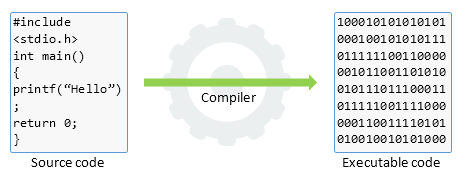
\includegraphics[width=0.8\textwidth]{compilation.png}
\end{figure}
\end{frame}

\begin{frame}
\frametitle{Compiled versus interpreted language}
\begin{figure}
\center
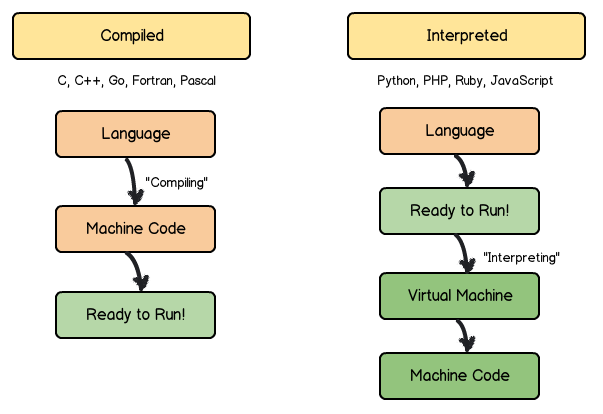
\includegraphics[width=0.8\textwidth]{compiled_vs_interp.png}
\end{figure}
\end{frame}

\section{Overview of C++}

\begin{frame}
\frametitle{Overview of the language}
\texttt{C++} is a compiled language designed to offer the programmer
high-level functionality, while retaining low-level capability.
\begin{itemize}
\item \texttt{C++} was written by Bjarne Stroustrup at Bell labs in 1980s
\item Based on the successful \texttt{C} language
\item Designed around the use of objects (object-oriented)
\end{itemize}
\end{frame}

\begin{frame}
\frametitle{Overview of the language}
\texttt{C++} is a compiled language designed to offer the programmer
high-level functionality, while retaining low-level capability.
\begin{itemize}
	\item \texttt{C++} was written by Bjarne Stroustrup at Bell labs in 1980s
	\item Based on the successful \texttt{C} language
	\item Designed around the use of objects (object-oriented)
\end{itemize}
	Objects in programming are similar in concept to real-world objects.
	They have \textit{states} and \textit{behaviors}. They are a useful
	concept for a number of reasons:
	\begin{itemize}
		\item modularity
		\item infromation-hiding
		\item code re-use
	\end{itemize}
	These features make \texttt{C++} great for large-scale software projects.
\end{frame}

\begin{frame}
\frametitle{Picking an Editor}
All computer code is typed up in some sort of text editor. Some text editors are better than others. For example Microsoft Word would be a terrible computer language text editor. Notepad could work, but there are much better editors out there. \\~\\
Some that I've seen students use before: 
\begin{itemize}
	\item emacs
	\item geany
	\item Vi/Vim
	\item Nano
	\item Sublime
	\item https://en.wikipedia.org/wiki/Comparison\_of\_text\_editors
\end{itemize}
\end{frame}

\begin{frame}
\frametitle{Opening the editor}
I'll let you choose which editor you would like to use later, for now we'll use vim. \\~\

Navigate to your class examples folder. In your terminal, type \texttt{vim HelloWorld.cpp}. This will create a file \texttt{HelloWorld.cpp} and open it in the vim editor. 

\end{frame}

\section{Hello World Program}

\begin{frame}
\frametitle{Simple Hello World Program}
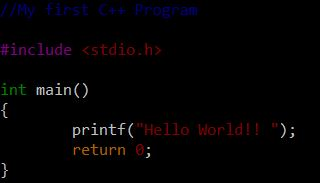
\includegraphics[width = 0.4\textwidth]{figures/HelloWorld.jpg}
\begin{block}{//}
Denotes that the rest of the line is a comment. The computer ignores comments. 
\end{block}
\begin{block}{\#include}
Tells the computer to include a particular package. In this case we are including the package stdio.h
\end{block}
\end{frame}

\begin{frame}
\frametitle{Simple Hello World Program}
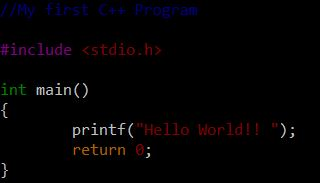
\includegraphics[width = 0.4\textwidth]{figures/HelloWorld.jpg}
\begin{block}{int main()}
This is where the program starts. It executes everything between the two curly braces \{ \}.
\end{block}
\begin{block}{printf();}
	\vspace{4pt} This is a function that takes some text (in this case "Hello World") and prints it to the terminal. \tiny (We will learn more about functions later)
\end{block}

\end{frame}


\begin{frame}
\frametitle{Simple Hello World Program}
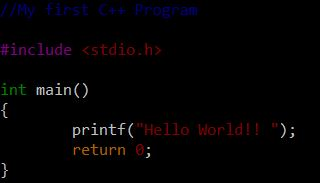
\includegraphics[width = 0.4\textwidth]{figures/HelloWorld.jpg}
\begin{block}{return 0;}
	This statement ends the program.
\end{block}
\begin{block}{;}
	Notice the semicolons at the end of the two statements, return 0; and printf(); above. These are critical, and belong at the end of most statements.
\end{block}

\end{frame}


\section{Running First Program}

\begin{frame}
\frametitle{Compiling}
Before the computer can execute/run our simple program we first have to compile it. Basically we put it through a process that translates it from our English text to computer understandable bits (ones and zeros) \\
\medskip
\begin{columns}[c] % The "c" option specifies centered vertical alignment while the "t" option is used for top vertical alignment

\column{.45\textwidth} % Left column and width
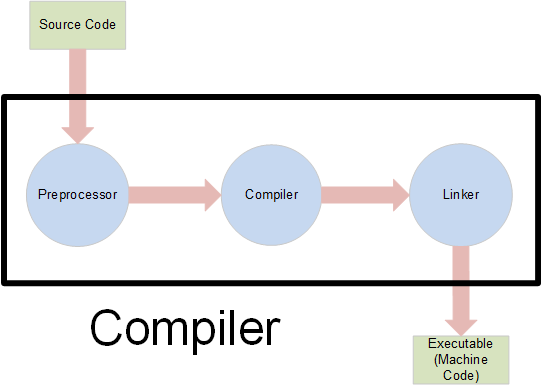
\includegraphics[width = 2in]{figures/compiler}

\column{.5\textwidth} % Right column and width
\begin{itemize}
\item Once your code has been successfully compiled it will now run on your machine.
\item We will learn more about the compiler in future lessons. 
\end{itemize}

\end{columns}

\end{frame}

\begin{frame}
\frametitle{Installing the g++ compiler}
\begin{minipage}[t]{0.45\textwidth}
	\flushleft
	\textbf{Windows 10: Bash on Ubuntu}
	\begin{enumerate}
		\item In your terminal, go home using the \texttt{cd \textasciitilde} command
		\item Type \texttt{sudo apt-get install g++} - This will install the g++ compiler.
		\item Check that it was installed correctly by typing \texttt{which g++} or \texttt{g++ --version}. The outputs should be similar to:
	\end{enumerate}
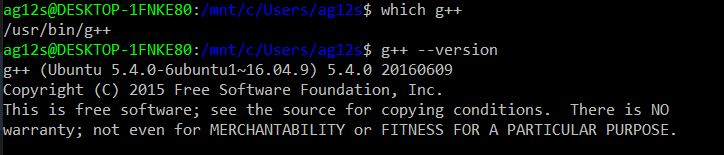
\includegraphics[width = \textwidth]{figures/g++Check}
\end{minipage}
\begin{minipage}[t]{.45\textwidth}
	\textbf{Mac Terminal}
	\begin{enumerate}
		\item In the Terminal type \texttt{g++}.
		\item If this alert box pops up, click "Install". You do not need Xcode unless you want Xcode.
		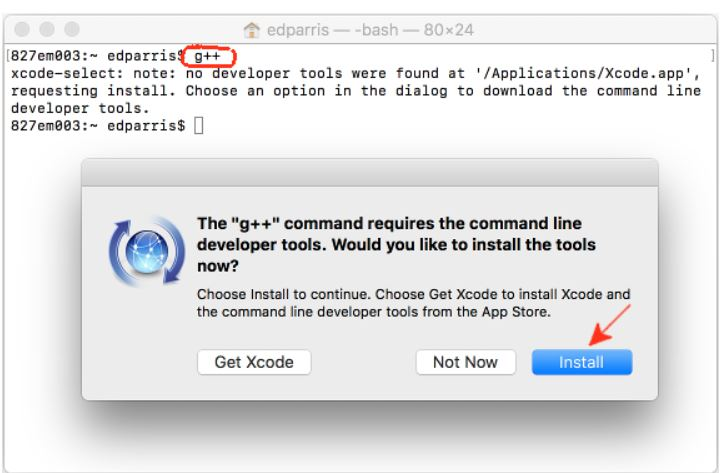
\includegraphics[scale = 0.25]{figures/g++Iterm}
		\item check that it has installed by typing \texttt{g++} in the terminal. This will return the error message \texttt{no input files}.
	\end{enumerate}
\end{minipage}
\end{frame}

\begin{frame}
\frametitle{Running our Program}
Now that we have installed the \texttt{g++} compiler, 
\begin{itemize}
\item In the terminal, navigate to the directory which contains our \texttt{HelloWorld.cpp} file
\end{itemize} 

\end{frame}

\begin{frame}
\frametitle{Running our Program}
Now that we have installed the \texttt{g++} compiler, 
\begin{itemize}
	\item In the terminal, navigate to the directory which contains our \texttt{HelloWorld.cpp} file
	\item Compile your program. Run the command \\
	\qquad \texttt{g++ HelloWorld.cpp -o HelloWorld}
\end{itemize} 
\end{frame}

\begin{frame}
\frametitle{Running our Program}
Now that we have installed the \texttt{g++} compiler, 
\begin{itemize}
	\item In the terminal, navigate to the directory which contains our \texttt{HelloWorld.cpp} file
	\item Compile your program. Run the command \\
	\qquad \texttt{g++ HelloWorld.cpp -o HelloWorld}
	\begin{block}{g++ HelloWorld.cpp -o HelloWorld}
		The \texttt{g++} command stands for compile. The Second option \texttt{HelloWorld.cpp} is the name of the file you want to compile. The third option \texttt{-o} stands for outfile and the fourth option  \texttt{HelloWorld} is what you wish the out file (executable file) to be called. Thus this command takes \texttt{HelloWorld.cpp} and creates a file called \texttt{HelloWorld} which is executable. 
	\end{block}
\end{itemize} 
\end{frame}

\begin{frame}
\frametitle{Running our Program}
Now that we have installed the \texttt{g++} compiler, 
\begin{itemize}
	\item In the terminal, navigate to the directory which contains our \texttt{HelloWorld.cpp} file
	\item Compile your program. Run the command \\
	\qquad \texttt{g++ HelloWorld.cpp HelloWorld}
	\begin{block}{g++ HelloWorld.cpp HelloWorld}
		The \texttt{g++} command stands for compile. The Second option \texttt{HelloWorld.cpp} is the name of the file you want to compile. The third option \texttt{-o} stands for outfile and the fourth option  \texttt{HelloWorld} is what you wish the out file (executable file) to be called. Thus this command takes \texttt{HelloWorld.cpp} and creates a file called \texttt{HelloWorld} which is executable.
	\end{block}
	\item Execute your program. Run the command.\\
	\qquad \texttt{./HelloWorld} 

\end{itemize} 
\end{frame}

\begin{frame}
\frametitle{Running our Program}
Now that we have installed the \texttt{g++} compiler, 
\begin{itemize}
	\item In the terminal, navigate to the directory which contains our \texttt{HelloWorld.cpp} file
	\item Compile your program. Run the command \\
	\qquad \texttt{g++ HelloWorld.cpp HelloWorld}
	\begin{block}{g++ HelloWorld.cpp HelloWorld}
		The \texttt{g++} command stands for compile. The Second option \texttt{HelloWorld.cpp} is the name of the file you want to compile. The third option \texttt{-o} stands for out file and the fourth option  \texttt{HelloWorld} is what you wish the out file (executable file) to be called. Thus this command takes \texttt{HelloWorld.cpp} and creates a file called \texttt{HelloWorld} which is executable.
	\end{block}
	\item Execute your program. Run the command.\\
	\qquad \texttt{./HelloWorld} 
	\begin{block}{./HelloWorld}
		The \texttt{./} command allows you to execute. It should be followed immediately by the executable file. No space.
	\end{block}
\end{itemize} 
\vspace{2pt}
Congratulations! You have just compiled and executed your program.
\end{frame}
\end{document}
